\section{The Motivating Example}
\label{section_motivating}

In this section, we formulate the problem of context-free path query evaluation, using a small graph and the classical \emph{same-generation query}~\cite{FndDB}, which cannot be expressed using regular expressions.

Let us have a graph database or any other object, which can be represented as a graph. The same-generation query can be used for discovering a vertex similarity, for example, gene similarity~\cite{GraphQueryWithEarley}. For graph databases, the same-generation query is aimed at the finding all the nodes at the same hierarchy level. The language, formed by the paths between such nodes, is not regular and corresponds to the language of matching parentheses. Hence, the query is formulated as a context-free grammar.

For example, let us have a small double-cyclic graph (see Figure~\ref{Example_Graph}). One of the cycles has three edges, labeled with $a$, and the other has two edges, labeled with $b$. Both cycles are connected via a shared node $0$.

\begin{figure}[h]
	\[
	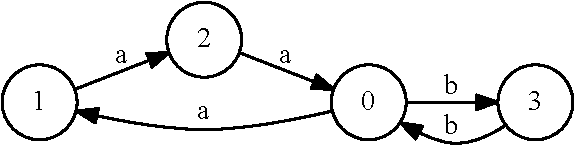
\includegraphics[width=7cm]{pictures/example_graph.pdf}
	\]
	\caption{An example graph.}
	\label{Example_Graph}
\end{figure}

For this graph, we have a same-generation query, formulated as a context-free grammar, which generates a context-free language \mbox{$L=\{a^n b^n~|~n \geq 1\}$}.

The result of context-free path query evaluation for this example is a set of node pairs \mbox{$(m, n)$}, such that there is a path from the node $m$ to the node $n$, whose labeling forms a word from the language $L$. For example, the node pair \mbox{$(0,0)$} must be in this set, since there is a path from the node $0$ to the node $0$, whose labeling forms a string \mbox{$w = aaaaaabbbbbb = a^6b^6 \in L$}.
